\documentclass[10pt,twocolumn]{article}
\usepackage[a4paper,margin=1.8cm,columnsep=0.6cm]{geometry}
\usepackage{amsmath,amssymb}
\usepackage{graphicx}
\usepackage{booktabs}
\usepackage[hidelinks]{hyperref}
\usepackage[font=small,labelfont=bf]{caption}
\usepackage{lmodern}
\setlength{\parskip}{2pt}

\title{\vspace{-1.2cm}\Large Escape rate, Lyapunov exponent and the uncertainty exponent\\of a latent-reasoning model}
\author{Euvel\\\small\url{https://github.com/euvel/eqr-transient-chaos}}
\date{\small 27 October 2026 --- technical note}

\begin{document}
\maketitle

\begin{abstract}
\noindent Recurrent reasoning models have fractal settle-time basins [1]. For the EqR Sudoku model we measure the two
rates behind them: the maximal Lyapunov exponent $\lambda_1$ and the escape rate $\kappa$ of the reasoning transient. We
then test the transient-chaos relation $f(\varepsilon)\propto\varepsilon^{\kappa/\lambda_1}$ for the fraction of
$\varepsilon$-close starting latents that settle at different loops. $\lambda_1 = 2.07$ per loop is a property of the
model (19 puzzles, uncorrelated with $\kappa$), whereas $\kappa$ varies 20-fold across puzzles. At true float64, with
$\varepsilon$ from $10^{-1}$ to $10^{-12}$, the measured exponent tracks $\kappa/\lambda_1$ on 9 puzzles (rank
correlation 0.92; 8 of 9 within $-23\%$ to $+19\%$), including 4 puzzles used only after a pre-registered first test.
Survival is exponential after a start-up of a few loops, and $f(\varepsilon)$ shows no steepening over 11 decades. For
this model the transient is therefore ordinary transient chaos with non-slim boundaries, not doubly transient chaos.
\end{abstract}

\begin{figure*}[t]
\centering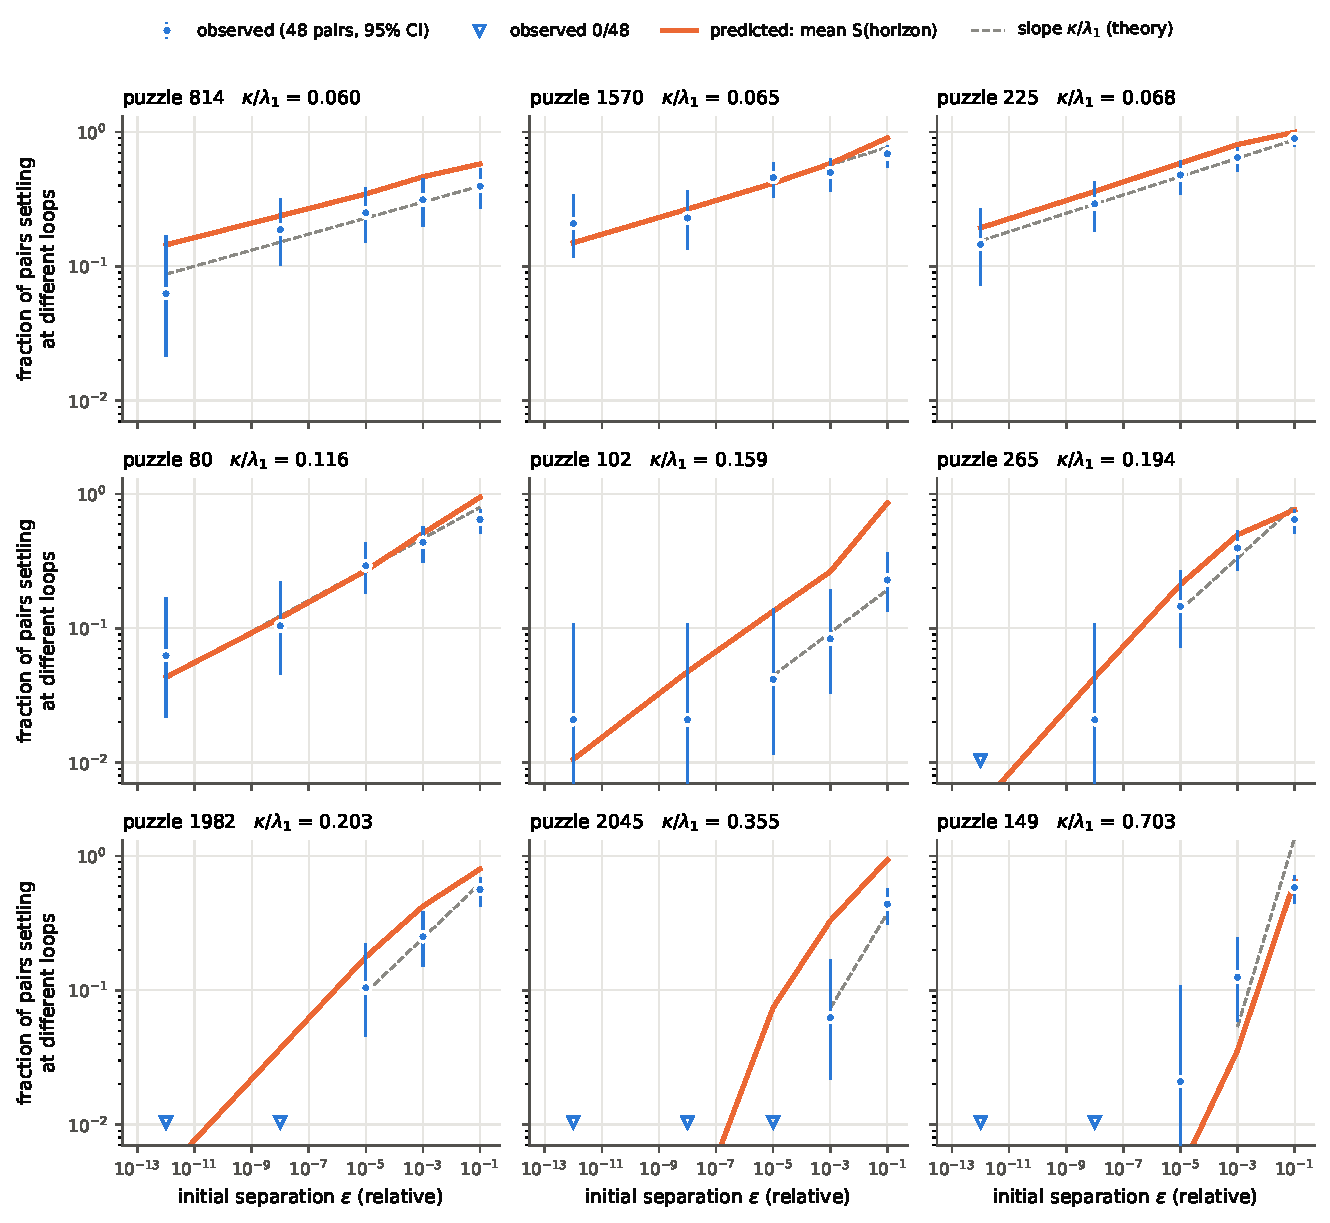
\includegraphics[width=0.86\textwidth]{../figures/fig1_eps_scaling.pdf}
\caption{Fraction of 48 $\varepsilon$-pairs settling at different loops (blue; 95\% Wilson intervals; triangles mark
0/48), the horizon prediction (orange), and a reference slope $\kappa/\lambda_1$ (grey). Panels are ordered by
$\kappa/\lambda_1$.}
\label{fig:eps}
\end{figure*}

\section{Background}
For an open chaotic system with escape rate $\kappa$ and maximal Lyapunov exponent $\lambda_{\max}$, the uncertainty
exponent $\alpha$ is defined by the fraction $f(\varepsilon)\sim\varepsilon^{\alpha}$ of initial conditions whose
outcome changes under a perturbation of size $\varepsilon$. It obeys $\alpha=\kappa/\lambda_{\max}$, and the boundary of
a 2D slice has dimension $2-\alpha$ [2--4]. Heuristically, a perturbation $\varepsilon$ grows to $O(1)$ after
$t_\varepsilon\approx\ln(1/\varepsilon)/\lambda_1$ loops, and the outcome changes only if the trajectory is still in the
transient by then: $f\approx S(t_\varepsilon)\approx e^{-\kappa t_\varepsilon}=\varepsilon^{\kappa/\lambda_1}$.

\section{Setup}
EqR Sudoku (checkpoint \texttt{locuslab/EqR-model}) via loopscape [1] at commit \texttt{16b52aa}, noise off, using the
demo slice: a random orthonormal 2-plane in the $97\times512$ latent $z_H$, with $z_L=0$. The settle time $T$ is the last
loop at which the decoded grid changes. $\kappa$ is an exponential fit to $S(k)=P(T>k)$ on a $40\times40$ map with cap
150, kept if $R^2\ge0.97$. $\lambda_1$ is the median over the 8 slowest trajectories of Benettin twins with QR ($K=4$,
offset $10^{-4}$). $\varepsilon$-pairs: a base point $z_0$ uniform on the slice and a partner
$z_0+\varepsilon\lVert z_0\rVert w$, with $w$ a random unit direction in the full latent, 48 pairs per level. These runs
use true float64. loopscape's float64 option silently runs in float32, and EqR's \texttt{rms\_norm} casts to float32;
both were patched and verified in-kernel (reported as loopscape\#1).

\section{Results}
\textbf{Rates.} Over 19 puzzles $\lambda_1$ has median 2.07 per loop (IQR 1.93--2.25), with no correlation with
$\kappa$ (Spearman $-0.01$) or with the median settle time ($-0.05$). $\kappa$ ranges from 0.049 to 1.08 per loop and is
unrelated to the human difficulty rating ($-0.14$). Since $\lambda_1$ is fixed by the model, a puzzle's fractality
$2-\kappa/\lambda_1$ is set by its escape rate alone.

\textbf{Exponent.} Fig.~\ref{fig:slope} compares the slope of $\log f$ against $\log\varepsilon$ with $\kappa/\lambda_1$
measured independently. Puzzle by puzzle the ratios are 1.17, 1.04, 1.16, 0.83, 1.19 (v5) and 0.77, 0.84, 0.90, 0.48
(v6). The outlier, 149 ($\kappa/\lambda_1=0.70$), rests on only 2 usable levels. Both runs registered this comparison as
a descriptive outcome without a pass bar.

\begin{figure}[t]
\centering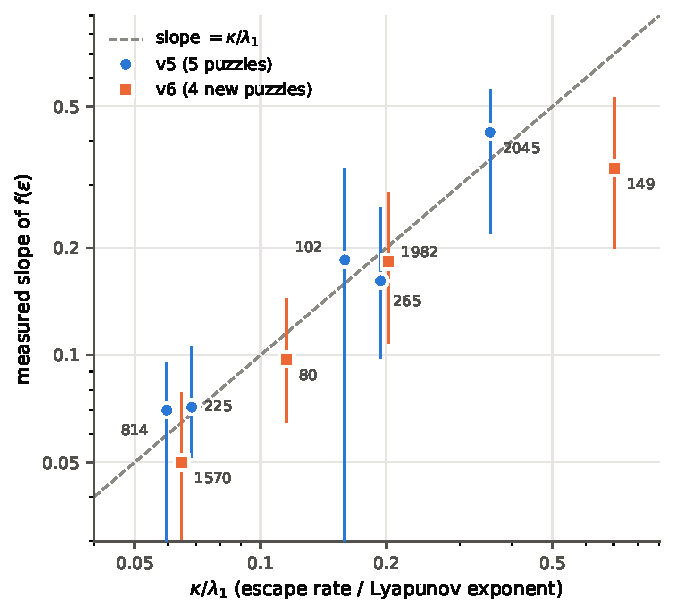
\includegraphics[width=0.92\columnwidth]{../figures/fig2_slope_vs_ratio.pdf}
\caption{Measured exponent of $f(\varepsilon)$ against $\kappa/\lambda_1$ (95\% bootstrap intervals over pairs). The
dashed line is $\alpha=\kappa/\lambda_1$. The v6 puzzles were not used in v5.}
\label{fig:slope}
\end{figure}

\textbf{Amplitude.} The horizon law $f\approx\langle S(\ln(0.1/d_0)/\lambda_1)\rangle$, where $d_0$ is the measured
separation after one loop, was the pre-registered prediction. In v5 it \emph{failed} its bar (61\% of points within
$2\times$, bar 70\%). Pooled over v5 and v6, 77\% of 31 points fall within $2\times$, and 87\% when each run's own
survival curve is used. The remaining bias is $\approx-20\%$, consistent with pairs that decorrelate yet settle on the
same loop. A post-hoc constant delay fitted on v5 was rejected out of sample in v6.

\textbf{Not doubly transient, not slim.} Lai et al.\ expect doubly transient chaos [1], in which the settling rate grows
in time and the boundaries become slim [5,6]. In discrete-time hazard fits on 13 maps, every puzzle shows a start-up of
2--6 loops followed by a constant exit rate. All 11 late-window fits are exponential, and the pooled rate changes by
$\times1.11$ per 50 loops (95\% upper bound $\times1.36$); puzzle 1216 holds 0.048 per loop from loop 8 to loop 93. The
local slopes of $f(\varepsilon)$ do not steepen: curvature $+0.006$ [$-0.09$, $+0.07$], and the largest small-$\varepsilon$
slope is 0.22.


\section{Limitations and open question}
These results cover one model, one task and one slice, with 9 puzzles for the exponent. Slopes come from 2--5 levels.
Survival is exponential within loop caps of 120--150. The relation $\alpha=\kappa/\lambda_{\max}$ does not distinguish
\emph{rough} from \emph{filamentary} boundaries [4]: that requires the cross-boundary Lyapunov exponent, which we did
not measure and which is the natural next experiment. Data, kernels, pre-registrations and a script for every number
are in the repository.

\small
\noindent\textbf{Acknowledgments.} Claude (Anthropic) collaborated on this work as an assistant. All decisions and
claims, and the responsibility for them, rest solely with the author.

\begin{thebibliography}{9}\setlength{\itemsep}{0pt}
\bibitem{lai26} J.~Lai, A.~Bao, J.~Quinn, W.~Gilpin, \emph{Fractal basins trap latent reasoning}, arXiv:2609.04963 (2026).
\bibitem{kg85} H.~Kantz, P.~Grassberger, Physica D \textbf{17}, 75 (1985).
\bibitem{lt11} Y.-C.~Lai, T.~T\'el, \emph{Transient Chaos}, Springer (2011), eq.~(5.13).
\bibitem{bl20} T.~B\'odai, V.~Lucarini, arXiv:2001.08871 (2020), eq.~(24).
\bibitem{m13} A.~E.~Motter, M.~Gruiz, G.~K\'arolyi, T.~T\'el, Phys.\ Rev.\ Lett.\ \textbf{111}, 194101 (2013).
\bibitem{c17} Y.~Chen, T.~Nishikawa, A.~E.~Motter, Phys.\ Rev.\ E \textbf{96}, 032215 (2017).
\end{thebibliography}
\end{document}
